\documentclass[a4paper,12pt, final]{report}
\usepackage{graphicx}
\usepackage{url}
%\usepackage[nomain,acronym,xindy,toc]{glossaries} % nomain, if you define glossaries in a file, and you use \include{INP-00-glossary}
%\makeglossaries
%\usepackage[xindy]{imakeidx}
%\makeindex
%\usepackage[section]{placeins}
\renewcommand\bibname{References}
\usepackage[utf8]{inputenc}
\usepackage{tikz}
\usepackage{subfig}
%\usepackage{algorithm2e}
%\usepackage{wrapfig}
\usepackage{epsfig}
\usepackage[demo]{graphicx}
\usepackage{float}
\usepackage{graphicx}
\usepackage{caption}
\usepackage{subcaption}
%\usepackage{hyperref}
\usepackage[hidelinks]{hyperref} % To Hide the box around links
\renewcommand\bibname{References}
%\usepackage{algorithm2e}
\usepackage{color}
\usepackage{textcomp}
\usepackage{acronym}
\usepackage[top=0.5in, bottom=1in, left=1in, right=1in]{geometry}
\usepackage{xcolor}
\definecolor{dark-red}{rgb}{0.4,0.15,0.15}
\definecolor{dark-blue}{rgb}{0.15,0.15,0.4}
\definecolor{medium-blue}{rgb}{0,0,0.5}

\newcommand{\BigO}[1]{\ensuremath{\operatorname{O}\bigl(#1\bigr)}}
\parindent 8pt
\begin{document}
  \thispagestyle{empty}
  \vspace*{1cm}
  {\centering     
  \textbf{\LARGE Software Prefetching for Graph Analytics}\\
  \vspace{1.20cm}
  %\it
  %\vspace{.5cm}
  %\rm
  \textbf{\large Dual Degree Stage 2 - February Report}\\
  \vspace{1cm}
  {Submitted in partial fulfillment of the requirements}\\
  \vspace{0.25cm}
  {for the }\\
  \vspace{1cm}
  \textbf{ Dual Degree Programme}\\
  \vspace{1.50cm}
  {by}\\
  \vspace{0.20cm}
  \textbf{\large Nayan Barhate}\\
  \vspace{0.25cm}
  \textbf{\large (Roll No. 180070037)}\\
  \vspace{1.8cm}
  {Under the guidance of}\\
  \vspace{0.20cm}
  \textbf{\large Prof. Virendra Singh}\\
    \vspace{0.30cm}
  \vspace{1.450cm}
    \begin{figure}[htb]
    \begin{center}
    
\includegraphics[height=1.5in,width=1.5in]{iitblogo.png}
    \end{center}
    \end{figure}

    
  {\textbf{Department of Electrical Engineering}}\\
  {\textbf{Indian Institute of Technology Bombay}}\\
  {\textbf{October 2022}}
 
 }
 
\renewcommand{\abstractname}{Acknowledgement}
\begin{abstract}
I express my gratitude to my guide Prof. Virendra Singh for providing me the opportunity
to work on this topic and support me throught the period of my work. I would also express my gratitude to the members of Computer Architecture and Dependable Systems Lab (CADSL)
for all the enlightening discussions in the lab meetings.
\\\\
\\\\
\\\\
Nayan Barhate\\
Electrical Engineering\\
IIT Bombay\\\

\end{abstract}
\clearpage 
\renewcommand{\abstractname}{Abstract} 
\abstract{
Graph analytics has applications in many different fields, including route optimization, computer networks, social networks, and recommendation engines. The capability of graphs to provide a visual representation of the links that exist between items enables their application in virtually every industry. Even when using applications from such a wide variety of domains, the performance of graph workloads is not even close to being optimal due to the poor locality that is displayed in caches. In most cases, the working set size in graph analytics is significantly greater than the memory capacity that is available on-chip. This results in a significant number of accesses to the primary memory. The primary obstacle to enhancing the performance of the system for graph analytics is lowering the amount of times it must access the main memory.

One way to optimise the utilisation of caches and cut down on accesses to main memory is to implement a cache replacement policy that is both effective and efficient. GRACE showcased that the current state-of-the-art cache replacement policies are unable to capture the extremely irregular memory access pattern displayed by graph applications. We propose a data-type aware cache management method as a means of making efficient use of the on-chip RAM that is currently available for graph analytics.

Through the implementation of an edge cache that partitions edge data from non-edge data, the purpose of this study is to bring the rate of missed accesses in graph applications down to a more acceptable level. In addition to this, we utilise software prefetching techniques to preload the edge cache with the data from the edge.
}

\tableofcontents
  \addcontentsline{toc}{chapter}{\listfigurename}
  \listoffigures
%  \printglossaries

%\newglossaryentry{ILP}
%{name = ILP,
%description = Instruction Level Parallelism}
\chapter{Introduction}
Graph applications are an important class of applications used to tackle a variety of problems, including path finding, web page searching, and recommendation systems, among others. Due to unanticipated industry development, graph processing is now essential. The graph analytics market was valued at \$600 million in 2019 and is projected to reach \$2.5 billion by 2024, expanding at a compound annual growth rate (CAGR) of 34\% over the forecast period\cite{graphMarket}. With the expansion of main memory in high-end servers, graphs are able to be stored in main memory. Even if shared memory systems outperform distributed memory systems, application performance is still constrained by irregular accesses in graph applications that render the memory hierarchy inefficient.

While graph applications have irregular memory accesses, an in-depth data-type-aware analysis of memory accesses can help us comprehend spatial and temporal locality from a data-type standpoint. Prior work that utilised graph reordering\cite{cite3}, prefetchers\cite{Basak2019AnalysisAO}\cite{cite5}, traversal\cite{cite6}, and cache policies\cite{cite7}\cite{poptcite8} to decrease memory hierarchy bottlenecks for graph applications. Basak et al.\cite{Basak2019AnalysisAO} presented a breakdown of the data kinds' accesses and hits at various cache hierarchy levels.

GRACE\cite{grace} has performed an analysis of the hits contribution and accesses contribution in order to further investigate performance enhancements. The majority of graph structure data hits were located at the L1-D cache level or in DRAM, while the majority of misses occurred at lower-level caches. However, it takes up a considerable amount of cache capacity for inclusive cache hierarchy. To prevent wasting cache capacity, we propose separating the structure/edge data of a graph from L2 and LLC, which enables property data to make efficient use of cache space.

\section{Background}
\subsection{Compressed Sparse Row (CSR) representation}
G(V,E) represents a graph G wherein we have V representing set of vertices and E
representing set of edges. An edge, $e \in E$ where $e=(u,v)$, indicates an edge from
source vertex u to destination vertex v for a directed graph. For an undirected graph,
it indicates an edge between vertices u and v. Commonly used formats for representing
graphs in memories include adjacency matrix and adjacency lists. An adjacency matrix
is efficient in finding a connection between vertices, u and v. The main disadvantage
of using an adjacency matrix is that it requires $\mathcal{O}(V^2)$ bits for storage. The storage
issue gets highlighted severely in the case of sparse data which does not have too many
connections between any pair of vertices. Adjacency list, on the other hand, is a more
compact representation than an adjacency matrix. However, it incurs pointer chasing
overheads while traversing the list through an address space because graph traversal
causes irregular memory access patterns.
Real-world graphs being sparse can be stored in a storage efficient manner using the
Compressed Sparse Row (CSR) format. Figure \ref{fig:CSR}, shows the CSR representation of
an example graph using the in-edges to a vertex. CSR uses three arrays:

\begin{itemize}
    \setlength\itemsep{0 em}
    \item \textbf{Offset array:} offset[i] stores the neighbour array offset for vertex id i .
    \item \textbf{Structure/Edge/Neighbour array:} Structure/Edge/Neighbour array: neighbour[j] (where $j \in$ offset$[i], $ offset$[i+1])$) stores the in (out) neighbour vertex ids of vertex i.
    \item \textbf{Property array(s):} property[i] stores partial or computed results for a vertex id i, e.g., The page rank application uses two property arrays wherein one property array stores the rank of all the vertices for the current iteration, while the other property array stores the rank of all vertices for the previous iteration.
\end{itemize}


\begin{figure}[h]
    \centering
    \input{CSR.tex}
    \caption{Compressed Sparse Row (CSR) graph using in-edges to a vertex}
    \label{fig:CSR}
\end{figure}

\textbf{Data type terminologies} frequently used for this work are listed below:
\begin{itemize}
    \setlength\itemsep{0 em}
    \item \textbf{Edge data:} Graph's data present inside the edge array
    \item \textbf{Property data:} Graph's data present inside the property array
    \item \textbf{Intermediate data:} Any data other than that of edge or property data
\end{itemize}

\begin{figure}[h]
    \centering
    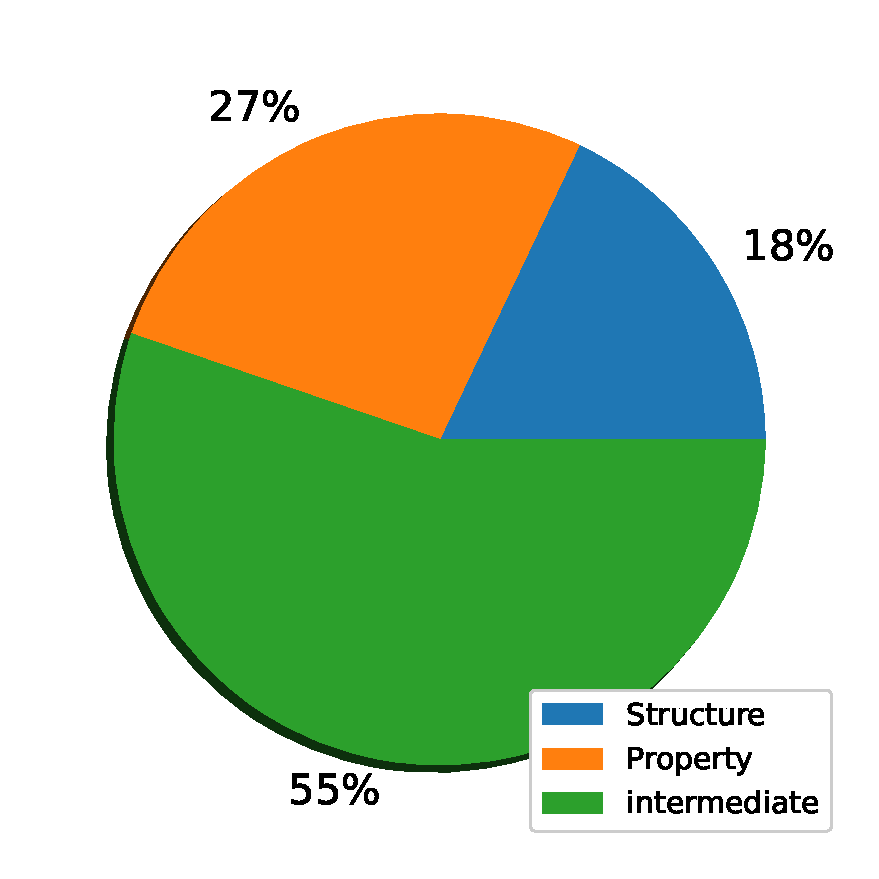
\includegraphics[width=0.4\linewidth]{access_dist.eps}
    \caption{Data type distribution for graph applications}
    \label{fig:my_label}
\end{figure}

\subsection{Graph Applications}
Because of the complexity and diversity of graph data, a large range of graph workloads
with varying computing behaviors exist. Modern graph applications are often categorized
into three types based on the type of computation % Graph Traversal

\begin{itemize}
    \setlength\itemsep{0 em}
    \item \textbf{Breadth-First Search (BFS)} is a traversal order that starts at a source vertex
and explores all the neighboring node. Before moving on to the next level, BFS
visits all vertices at the current depth (distance from the source vertex). Since BFS
is so fundamental, it is frequently implied in other graph algorithms.

    \item \textbf{Single-Source Shortest Paths (SSSP)} algorithm computes the shortest paths
from a given source vertex to every other connected vertex. The distance between
two vertices is computed as the minimum sum of edge weights along the path that
connects the two vertices.

    \item \textbf{PageRank(PR)} calculates the PageRank score for each vertex in a graph. The
output (PR) for a vertex v with a damping factor d is as follows:
$$PR(v) = \frac{1-d}{|V|}+\sum_{u\in N-(v)}\frac{PR(u)}{|N^+(u)|}$$
\end{itemize}


\subsection{Characteristics of Graph Datasets and Applications}
\subsubsection{Power-law distribution}
Many real-world graph datasets have been found to be following a power-law degree
distribution of vertices, where only a few fractions of vertices contribute to most of the
edges of a graph

\subsubsection{Community structure}
Vertices in real-world graphs form communities [12] that can help exploit the spatial
locality of nearby vertices to be visited soon when placed together in memory.


\subsubsection{Irregular accesses}
In an iteration, graph processing involves accessing the offset array first and then access-
ing edge array data followed by property array data. It makes the accesses be of type
A[B[C[i]]], which are known to be highly irregular and not cache-friendly.

\subsection{Push or pull computation}
Vertex-centric processing is known to execute the applications in two ways:

\begin{itemize}
    \setlength\itemsep{0 em}
    \item \textbf{Push-type computation} A vertex pushes the value to its out-neighbours. In this case, every pushing vertex must acquire a lock to the destination vertex that it is pushing (writing) data to some destination vertex.

    \item \textbf{Pull-type computation} A vertex pulls (reads) the value from its in-neighbors to calculate the property for the current vertex. In-neighbors need not acquire locks to the current vertex because it only reads the values from its neighbors.
\end{itemize}

\subsection{Cache affinity for different data types}
In vertex-centric processing the graph applications execute as:
\begin{itemize}
    \setlength\itemsep{0 em}
    \item For a vertex v get the information about its Ni (in-neighbours) (or) No (outneighbours).
    \item For each in/out (Ni/No) neighbour pull/push the value for vertex v from/to the
desired neighbour.
\end{itemize}
In every iteration, the property of a vertex v is computed using its neighbors. Table 1.1
lists the different types of cache locality existing for a graph-specific data type using the
knowledge about how the graph applications are accessing the data.

\begin{table}[]
    \centering
    \begin{tabular}{|c||c|c|} \hline
         Array  & Temporal locality & Spatial Locality  \\ \hline\hline
         Vertex & No & Yes \\ \hline
         Edge  & No & Yes\\ \hline
        Property & Yes &  No  \\\hline
    \end{tabular}
    \caption{Existence of locality for Vertex ordered schedule with graphs stored in CSR
format}
    \label{tab:my_label}
\end{table}

\section{Thesis organization}
Chapter \ref{chap:relatedWorks} gives the various works related to improving graph application's performance
on multi-core architectures. It motivates this work and provides results to show the
scope of the work. Chapter \ref{chap:proposal} provides the information related to the proposal, necessary
modifications required (hardware and software)
Chapter \ref{chap:conclusion} concludes this work with the future work.

\chapter{Related work}\label{chap:relatedWorks}
\section{Literature survey}
\subsection{Characterization}
Many researchers have tried to figure out the bottlenecks of traditional CPU architectures. They 
have shown that these applications are memory-bound as they suffer
from a large number of memory accesses, and memory bandwidth is not fully utilized due
to irregular serial accesses.

\subsection{Reordering}
Prior work has worked with sibling and neighbor relationships between the vertices
to improve the cache locality, which can reduce the cache misses, thereby improving the
system's performance. Although this work provides reasonable speedup benefits, the
overhead associated with reordering time is signifficant. V. Balaji et al. \cite{poptcite8} pointed
out that using the power-law characteristics demonstrated by real-world graphs, we can
simplify the reordering algorithm. This will reduce the reordering cost and help achieve
speedups comparable to that achieved by more formal graph reordering techniques. However, these solutions achieve speedup using algorithmic renaming of vertices only. Vertices
accessed together frequently are placed together in memory as close as possible by these
lightweight reordering algorithms.

\subsection{Cache policies}
Aamer et al. proposed DRRIP\cite{DRRIP} for mixed access patterns: recency-friendly and
thrashing patterns commonly observed at the LLC. It uses Set dueling to decide
between the two replacement policies, SRRIP and BRRIP. Faldu et al. \cite{cite7} proposed the
Last-level cache policy taking into account the power-law characteristics exhibited by
the vertices of a real-world graph. It gives priority to high-degree nodes over low-degree
nodes so that the latter is the most-suited eviction candidate in a cache replacement
policy. This method also required reordering the vertices in software before running the
application to make high, medium, and low reuse regions of the property array according
to their degrees.

Graph processing frameworks store both original and transposed representations for
both push or pull-type computation phases of an application. This transposed graph
information helps Belady's-Optimal Cache Replacement Policy. P-OPT\cite{poptcite8} determined
how far in the future a particular cache block will be again accessed using the information
from the transposed graph.

\subsection{Prefetching}
\subsubsection{Hardware Prefetching}
Previous work, Indirect memory prefetcher (IMP)\cite{IMP} which used hardware prefetcher
to prefetch the requests A[B[i]]. However, this approach is a pure hardware solution and
requires training a Prefetch Table for indirect memory access patterns.
DROPLET\cite{cite4} is a data-aware prefetcher that requires the memory subsystem to know
the data type, i.e., edge, property, or intermediate. It helps the prefetcher to prefetch
the property data request when the edge data request returns on-chip. This approach
effectively improves the hit rates for the least utilized L2 cache but does not train the
prefetcher.

Prodigy\cite{prodigy} is an L1-D prefetcher designed to work on graph-based data.
Prodigy prefetches into all the data lists of CSR format. It requires
compiler support to form a Data-Indirection Graph(DIG) which is used
to store address bounds and the relation between different data lists.
Data-Indirection Graph is a common data structure for the graphs of any
type of representation. Prodigy requires the dataset/graph to be divided
into multiple lists (like CSR format) to access the bounds of the lists and
forms a Data-Indirection Graph. Each node of DIG stores the node id for
identification of a list, base addr, capacity and data size are used to find
out address bounds(first and last address) of the list represented by the
node. The edges of DIG represent the type of indirection between the
lists, edges also tell the order of prefetching. An edge from vertex list to
edge lists conveys that edge list elements are prefetched after the vertex
list is prefetched. Each graph has at least one trigger node which has a
self-loop over it called trigger edge. Whenever demand access comes to
an address, prefetching start only from its trigger edge and continues till
the leaf node of DIG.

DROPLET\cite{droplet} is a data-aware prefetcher that requires the memory subsystem to know
the data type, i.e., edge, property, or intermediate. It helps the prefetcher to prefetch
the property data request when the edge data request returns on-chip. This approach
eectively improves the hit rates for the least utilized L2 cache but does not train the
prefetcher.

\subsubsection{Software Prefetching}
S. Ainsworth, et. al. \cite{softPrefetch} developed a novel compiler pass to automatically
generate software prefetches for indirect memory
accesses, a special class of irregular memory accesses often
seen in high-performance workloads. For indirect access like $A[B[i]]$, the addresses accessed
in $A$ array are data-dependent, a hardware
stride prefetcher will be unable to discern any pattern, so
will fail to accurately prefetch them. However, future memory
access addresses can easily be calculated in software due
to being able to look ahead in $B$ array.
For timely prefetch, we prefetch $A[B[i + $offset$]]$ and $A[i+2\times$ offset$]$. In case of indirect access, there is a intermediate load in the prefetch code and we need to ensure that the address is in bounds to avoid any faults. This is done by a simple if condition. Software prefetching achieves 3.7x speedup on in-order Intel Xeon Phi machine and 1.3x speedup on out-of-order ARM Cortex-A57 machine. 


\subsection{Cache Utilization in Graph Applications}
In previous work, \cite{grace} pointed that for a system with 3 levels of inclusive cache hierarchy with 32KB 8 way L1 cache, 256KB 8 way L2 cache and 8MB 16 way LLC cache showcased that hit rate for edge data for L1 is 78.2\%, 1.8\% for L2 and LLC combined and the remaining 20\% hits at DRAM. Property data gets 55.3\% hits at L1-D, 4.2\% at L2, 20.2\% at LLC and
remaining 20.3\% hits from DRAM. Table \ref{tab:avgHits} summarizes average hits contribution for all data types from all memory hierarchy levels. 

Access contributions for all of the data types are comparable to each other at all levels of cache.

In a phasewise execution of PR application, it was found that the cache occupancy for edge data variers between 7\%-94\% for L2 cache and 11\%-73\% for LLC. Although edge array
data occupies significant cache space at L2 and LLC, the L2 and LLC still fails to capture
any significant locality present in edge array data accesses.

\begin{table}[h]
\centering
\begin{tabular}{|c||c|c|c|c|}
\hline
\textbf{Data type}    & \textbf{\begin{tabular}[c]{@{}c@{}}L1-D\\ \%\end{tabular}} & \textbf{\begin{tabular}[c]{@{}c@{}}L2\\ \%\end{tabular}} & \textbf{\begin{tabular}[c]{@{}c@{}}LLC\\ \%\end{tabular}} & \textbf{\begin{tabular}[c]{@{}c@{}}DRAM\\ \%\end{tabular}} \\ \hline\hline
\textbf{Edge} & 78.2 & 0.3 & 1.5 & 20\\ \hline
\textbf{Property} & 55.3 & 4.2 & 20.2 & 20.3\\ \hline
\textbf{Intermediate} & 92.7 & 1.2 & 2.9 & 3.1             \\\hline
\end{tabular}
\caption{Summary of average hits for each data type at all cache levels and memory}
\label{tab:avgHits}
\end{table}



\chapter{Motivation}


\section{Experiments Conducted}
\subsection{Memory Hierarchy Usage - GRACE}
\begin{figure}[!htb]
    \centering
    \subfloat[\centering Baseline ]{{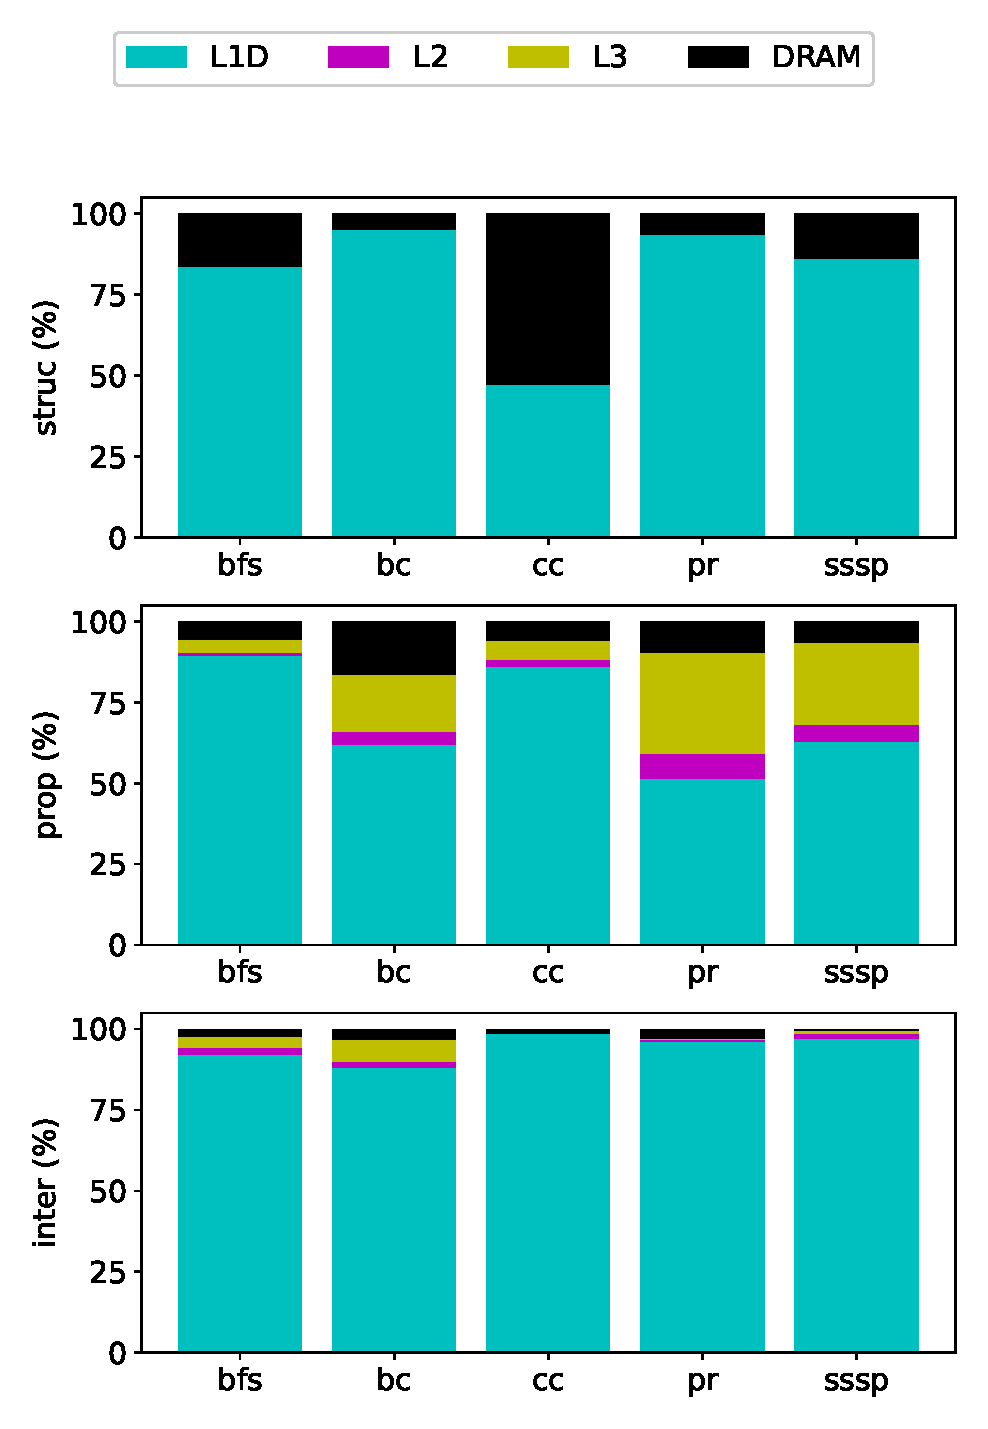
\includegraphics[width=0.45\linewidth]{no_grace_stack.eps} }}%
    \qquad
    \subfloat[\centering GRACE]{{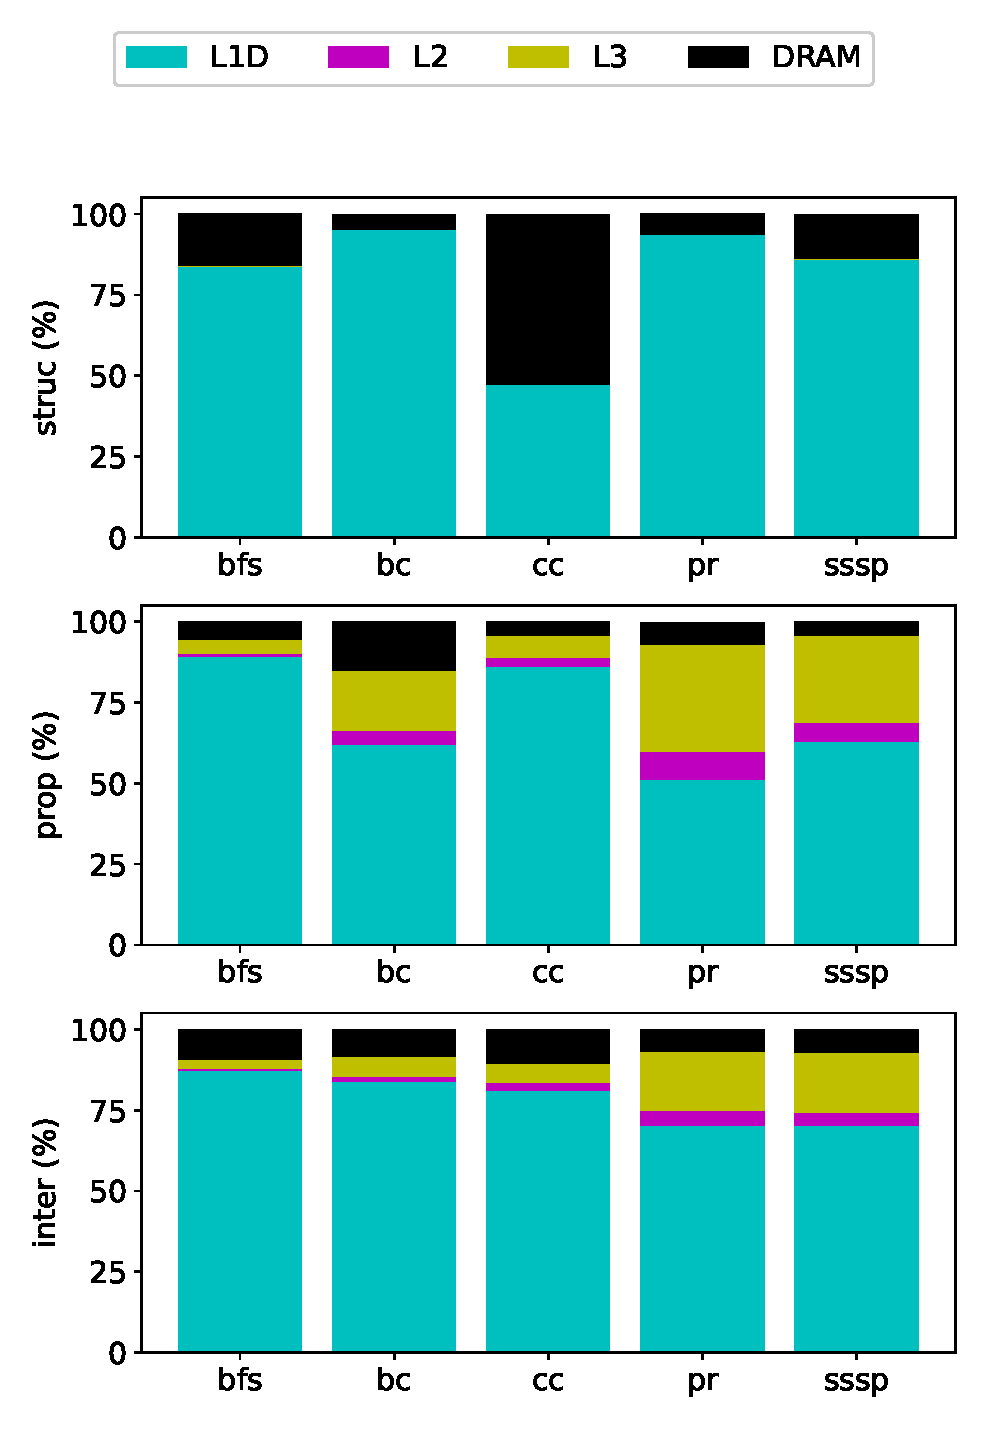
\includegraphics[width=0.45\linewidth]{grace_stack.eps} }}%
    \caption{Hit contribution of different data type for LiveJournal dataset}%
    \label{fig:stacked_bar_grace}
\end{figure}

In GRACE, edge data is bypassed from L2 and LLC freeing space for property and intermediate data, but from
figure \ref{fig:stacked_bar_grace} we can infer that the memory hierarchy usage for property data remains almost the same and reduces the L1 hit rate for the intermediate datatype. In case of property data GRACE increased the L2 hit rate by $2\%$ while the structure L1 hit rate remains the same. This shows that the L2 cache is still underutilised by GRACE and can be improved upon.
\subsection{Perfect Prefetching}
\begin{figure}[!htb]
    \centering
    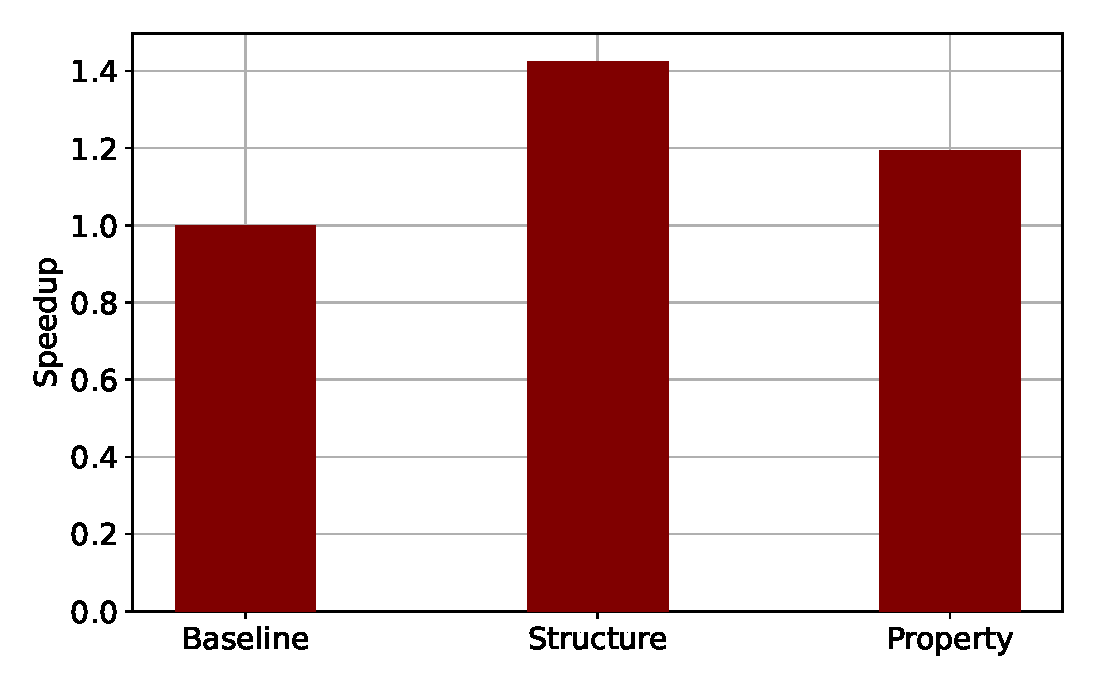
\includegraphics[width=0.6\linewidth]{perfect_L1_cache.eps}
    \caption{Perfect Prefetching for different data types}
    \label{fig:my_label}
\end{figure}
In this experiment, we modeled a perfect data-aware prefetcher for structure and property data. This prefetcher prefetched in a timely manner into the L1 cache. We assumed a separate 32KB 8-way cache for each data type. Prefetching Structure data perfectly gave $42\%$ speedup while prefetching property data gave $19\%$ speedup.

\subsection{Sensitivity analysis of Edge Cache and Property Cache}
\begin{figure}[!htb]
    \centering
    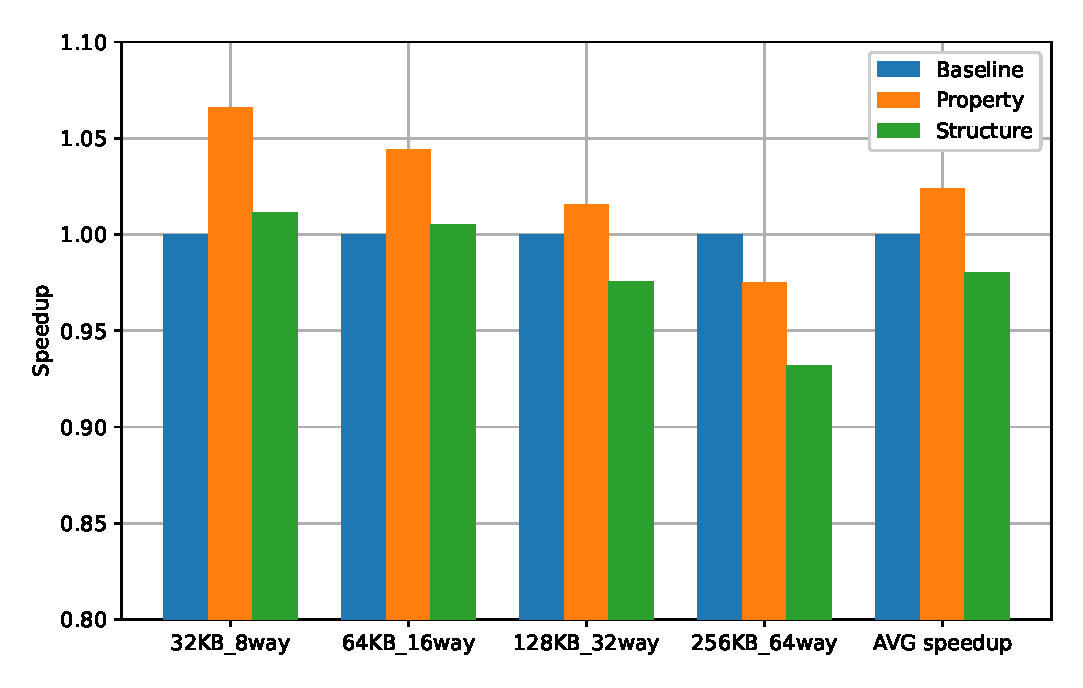
\includegraphics[width=0.8\linewidth]{sensitivity.eps}
    \caption{Sensitivity analysis of Edge Cache and Property Cache}
    \label{fig:my_label}
\end{figure}
In this experiment, we modeled separate 32KB 8-way cache for each data type and changed the size of one keeping the other caches constant. For structure and property cache, we observed that increasing the cache size led to speed down and gave maximum speedup for 32KB 8-way. 


GRACE\cite{grace} showcased that Edge data rarely gets a hit at lower-level caches after missing the data at L1-D cache. L2 cache does not provide any significant hits to edge data type. Without receiving any significant hits at lower-level caches, edge data still occupies
significant cache space. Sensitivity analysis of lower-level caches indicates that property data hit rate can improve with increased cache space. Property data gets significant hits at LLC. This leads us to our proposal to address these observations.

\chapter{Proposal}\label{chap:proposal}
\section{Proposed Architecture}
\begin{figure}[h]
    \centering
    \input{propsedarch}
    \caption{Propsed Architecture with Edge cache}
    \label{fig:propsedArch}
\end{figure}



Bypassing the edge data directly to DRAM greatly benefits the system irrespective of the cache replacement policy. To further reap the benefits we add a edge cache to separate edge and non-edge accesses. The freed space in L2 and LLC can be used by other data accesses like property data. Property data utilizes the L2 and LLC space better than edge data. Any edge access is sent directly to edge cache after address translation. If it incurs a miss the access is sent to DRAM. In case of any non-edge access, the accesses follows the traditional flow from L1 to L2 to LLC to DRAM. 

% explain the architecture shorly

\section{Hardware Modifications}
By passing the edge data leaded directly to 16\% speedup. Property data's L2 and LLC hit increases with increase in the size that is available to the data unlike edge data. Edge data during a PR algorithm occupies around 7-93\% in L2 and 10-72\% in LLC cache. Storing Edge data in a separate cache will give the other data like property some space to \cite{grace}
Since Edge cache is at the same level as L1D cache, the processor and directly get the data in this cache without adding any other overhead. This cache does not affect the critical path as it operates parallel to L1D cache.


% \subsection{Access flow in case of Edge data}


\section{Software Modifications}
Since for a static graph its offset and edge array is read-only. As suggested in \cite{softPrefetch}, we can add prefetch instruction in the code to get the edge data directly in the Edge cache. In case of indirect access, there is a intermediate load in the prefetch code and we need to ensure that the address is in bounds to avoid any faults. This is done by a simple if condition. If the edge offset is known as in ranged indirection, we can prefetch the direct address without any bound check.

To identify edge data, the operating system and graph processing framework will be modified. The graph processing framework includes an allocation layer for graph data. As implemented in prior work\cite{grace}, we modified the functionality of \texttt{malloc} to identify edge data at the graph data allocation layer. The functionality of \texttt{malloc} is modified to make it easier to populate a bit in the page permission field of each and every page in the page table. This extra bit is set to logic '1' for edge data and logic '0' for non-edge data by the modified \texttt{malloc}. Since we already have a few unused bits in the page permission field (for X86 ISA), we do not need to add an additional bit to the page table to accommodate the same.

\section{Cache Coherency Challenges}
Edge data for static graphs can only be read. No core will therefore modify the cache blocks containing edge data. A core (such as C1) may require edge data that is already present in the private cache of another core (e.g., C0). In a typical scenario, the core C1 would receive an LLC cache hit for the requested cache block. In our proposed scenario, the C1 core would not be able to locate the requested cache block in the LLC. Consequently, core C1 will acquire the cache block from main memory, eliminating the need to track cache blocks containing edge data at the tag directory in order to maintain cache coherency.


\chapter{Conclusion \& Future Work}\label{chap:conclusion}
\section{Conclusion}
Graph processing has irregular memory accesses, which heavily penalizes the performance
in comparison with sequential accesses. Analysis of different types of memory accesses
involved in graph processing is essential for understanding the scope to improve cache
hierarchy utilisation. A detailed characterization of the hits contribution and accesses
contribution at every cache level showed that edge data present in the graph's CSR representation does not benefit from the presence of lower-level caches and, at the same time,
occupies a significant cache space. Sensitivity analysis for lower-level caches shows that
if cache space for property data increases, it can harness better locality. Bypassing the
edge data from lower-level caches provides more cache space to the property data. In order to fully reap the benefits of edge cache, we prefetch the edge data into the cache using software prefetch instructions.
Prefetching Indirect access is better handled in software as their addresses are well known to compiler.




\section{Future Work}
The Final aim of this work is to reduce the miss rate observed in graph application due to its random accesses, therby increasing the performance of the system. 
Future work includes the following:
\begin{itemize}
    \setlength\itemsep{0 em}
    \item To modify the GRACE code to incorporate edge cache in SniperSim
    % \item Run experiments and analyse the current work in order to find where
% the issue persists in cache hierarchy.
    \item Modify the code to incorporate software prefetching
    \item Tune the prefetching lookahead distance (offset)
\end{itemize}



\bibliographystyle{ieeetr}
\bibliography{thesisTemplate}{}
\end{document}
